
\label{sec:Theorie}
\section{Zielsetzung}

In diesem Versuch wird die Dipolrelaxation eines Ionenkristalls untersucht,
wobei sowohl die charakteristische Relaxationszeit der Dipole als
auch die Aktivierungsenergie des Materials experimentell bestimmt werden.

\section{Theorie}
Ein Ionenkristall ist im Allgemeinen eine periodische Anordung aus positiv geladenen
Kationen und negativ geladenen Anionen, die aufgrund der elektrostatischen Anziehung
eine Ionenbindung eingehen und somit einen Kristall bilden. Bringt man anstelle
der einfach geladenen Kationen auch doppelt geladene Kationen, wie beispielsweise
$\ce{Sr^{++}}$ ein, so kommt es aufgrund der notwendigen Ladungsneutralität des Kristalls
zu Leerstellen an den Stellen wo üblicherweise ein einfach positiv geladenes Kation
sitzt. Dies ist in Abbildung \ref{fig:ion} dargestellt.
\begin{figure}
  \centering
  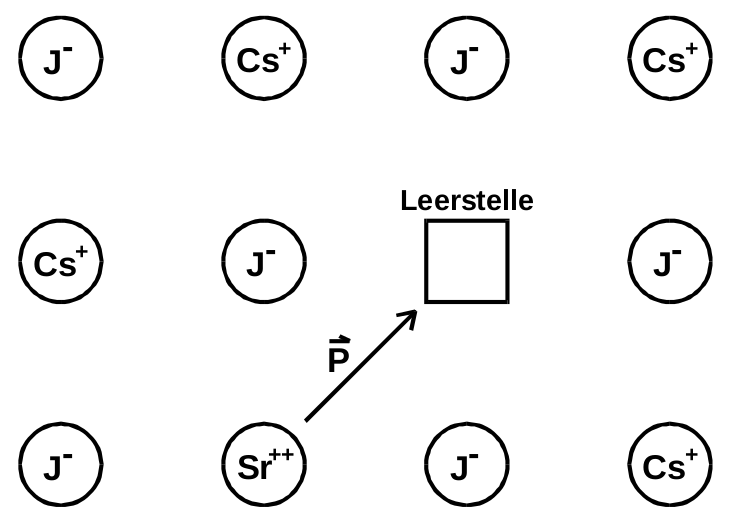
\includegraphics[width=8cm]{ion.png}
  \caption{Aufbau eines CsI-Kristalls mit permanenten Dipolen durch Dotierung mit Strontium \cite{skript}.}
  \label{fig:ion}
\end{figure}
Die Leerstellen bilden dabei mit den zweifach geladenen Kationen permanente
Dipole im Kristall aus, welche an die Symmetrie des Gitters gebunden sind und
somit nur diskrete Werte und Richtungen erlauben. Diese sind jedoch statistisch verteilt,
sodass es keine Vorzugsrichtung und somit auch kein makroskopisches Dipolmoment gibt. \\
Durch die thermische Bewegung ist es den Leerstellen, welche die Aktivierungsenergie
$W$ besitzen um das Gitterpotential zu überwinden, möglich sich im Kristall zu bewegen,
was eine Richtungsänderung des Dipols ermöglicht. Da diese Aktivierungsenergie
durch die thermische Energie der Dipole aufgebracht wird, ist der Anteil dieser
beweglichen Leerstellen gemäß der Boltzmann Statistik gegeben. Daraus
lässt sich die Relaxationszeit, welche die mittlere Zeit zwischen zwei Umorientierungen
eines Dipols bezeichnet, über
\begin{equation}
  \tau(T)=\tau_0\exp{\frac{W}{\symup{k_B}T}}
  \label{eqn:tau}
\end{equation}
berechnen. Dabei bezeichnet $\tau_0$ die charakteristische Relaxationszeit, welche den Grenzwert
der Relaxationszeit bei hohen Temparaturen angibt $\tau_0=\lim_{T \to \infty}\tau(T)$. \\
Wird ein solcher Dipol einem externen elektrischen Feld ausgesetzt, so richtet sich
ein Teil $y(T)$ der Dipole, welcher durch die Langevin-Funktion gegeben ist in Richtung des Feldes
aus. Dafür muss die Zeit, in der das Feld angelegt ist, groß sein gegenüber
der Relaxationszeit.
Unter der Annahme $pE\ll\symup{k_B}T$, wobei $p$ das Dipolmoment bezeichnet und $E$ die
Stärke des Feldes, lässt sich diese Funktion zu
\begin{equation}
  y(T)=\frac{pE}{3\symup{k_B}T}
  \label{eqn:anteil}
\end{equation}
nähern. Kühlt man den Kristall anschließend bei eingeschaltetem Feld zügig ab, so lässt sich
die Anzahl der Dipole "einfrieren". Wird nun eine konstante Heizrate
\begin{equation}
  b:=\frac{\symup{d}T}{\symup{d}t}
  \label{eqn:hrate}
\end{equation}
angelegt, so beginnen die Dipole zu relaxieren und es fließt ein Relaxationsstrom mit der Stromdichte
\begin{equation}
  j(T)=y(T_p)\cdot p \cdot \frac{\symup{d}N}{\symup{d}t} \:,
\end{equation}
wobei $y(T_p)$ den Anteil der Dipole bezeichnet, welche vor der Abkühlung ausgerichtet waren,
$p$ das Dipolmoment und $\frac{\symup{d}N}{\symup{d}t}$ die Rate, mit der die Dipole relaxieren.
Diese Relaxationsrate lässt sich analog zum Radioaktiven Zerfall berechnen, mit der temperaturabhängigen
Relaxationszeit $\tau(T)$ und der Annahme, dass die Rate proportional zu der Anzahl $N$ der noch nicht relaxierten
Dipole ist. Hieraus lässt sich die Differentialgleichung
\begin{equation}
  \frac{\symup{d}N}{\symup{d}t}=-\frac{N}{\tau(T)}
  \label{eqn:DGL}
\end{equation}
herleiten, aus welcher durch Integration die Formel
\begin{equation}
  N(T)=N_p \exp{\Big(-\frac{1}{b}\int_{T_0}^{T} \frac{\symup{d}T´}{\symup{d}t}\Big)}
\end{equation}
folgt, mit der Anzahl $N_p$ der vor der Abkühlung augerichteten Dipole
und der entsprechenden Temperatur $T_0$ vor dem Abkühlen. Unter Verwendung
der Gleichungen \eqref{eqn:tau} und \eqref{eqn:anteil} folgt damit insgesamt für die
Relaxationsstromdichte $j(T)$ die Formel
\begin{equation}
  j(T)=\frac{p^2E}{3k_BT_p}\frac{N_p}{\tau_0}  \exp{\Big(-\frac{1}{b}\int_{T_0}^{T}
  \symup{d}T´\exp{\Big(-\frac{W}{k_BT´}\Big)}{\symup{d}t}\Big)}
  \exp{-\Big(\frac{W}{k_BT}\Big)} \:.
  \label{eqn:stromd}
\end{equation}
Da sich im Anfangsbereich der Stromkurve für das Integral $\int_{T_0}^{T} \symup{d}T´\,\exp{(-\frac{W}{k_bT´})} \approx 0$
ergibt, lässt sich dort die Gleichung über
\begin{equation}
  j(T)\approx \frac{p^2E}{3k_bT_p}\frac{N_p}{\tau_0} \exp{\Big(-\frac{W}{k_BT}\Big)} \:
  \label{eqn:stromnäherung}
\end{equation}
nähern. \\
Alternativ lässt sich die Aktivierungsenergie $W$ auch aus dem gesamten Stromverlauf bestimmen,
indem die Polarisation $P$, also das Gesamtdipolmoment pro Volumeneinheit betrachtet wird, welche
proportional zur Anzahl der ausgerichteten Dipole ist. Diese erfüllt dabei die Gleichung
\begin{equation}
  \frac{\symup{d}P}{\symup{d}t}=-\frac{P(t)}{\tau(T(t))} \: ,
  \label{eqn:PolDGL}
\end{equation}
wobei durch die zeitliche Änderung der Polaristation ein Strom der Form
\begin{equation}
  I(t)=F\, \frac{\symup{d}P}{\symup{d}t}
\end{equation}
resultiert mit dem Probenquerschnitt $F$. Durch Integration ergibt sich hieraus die Formel
\begin{equation}
  \tau(T)=\frac{\int_T^\infty I(T´)\symup{d}T´}{b\,I(T´)} \: .
\end{equation}
Mit der Formel \eqref{eqn:tau} ergibt sich somit
\begin{equation}
  \frac{W}{\symup{k_B}T}=\text{ln}\frac{\int_T^\infty I(T´)\symup{d}T´}{\tau_0\,b\,I(T´)} \: ,
  \label{eqn:integral}
\end{equation}
sodass sich aus der Propotionalitätskonstante zwischen $\text{ln}\frac{\int_T^{T^*} I(T´)\symup{d}T´}{\tau_0\,b\,I(T´)}$
und $\frac{1}{T}$ der Wert der Aktivierungsenergie ergibt. Für die obere Integrationskonstante $T^*$
gilt dabei $I(T^*)\approx0$. \\
Um zudem den Wert von $\tau_0$ zu bestimmen wird die Lage des ersten Maximums der Stromkurve betrachtet.
Durch die Verschiebung zu Gitterplätzen übernächster Nachbarn enstehen auch weitere Maxima,
welche für diesen Wert jedoch nicht relevant sind. Durch Differentiation der
Gleichung \eqref{eqn:stromd} ergibt sich diese Lage
zu
\begin{equation}
  \tau_{\text{max}}(T_{\text{max}})=\frac{k_BT^2_{\text{max}}}{bW} \: ,
  \label{eqn:taumax}
\end{equation}
woraus sich durch einsetzen des Wertpaares $\tau_{\text{max}}(T_{\text{max}})$ und
$T_{\text{max}}$ in \eqref{eqn:tau} die charakteristische Relaxationszeit $\tau_0$ ergibt.
